%%%%%%%%%%%%%%%%%%%%%%%%%%%%%%%%%%%%%%%%%%%%%%%%%%%%%%%%%%%
% --------------------------------------------------------
% Tau
% LaTeX Template
% Version 2.4.1 (22/05/2024)
%
% Author: 
% Guillermo Jimenez (memo.notess1@gmail.com)
% 
% License:
% Creative Commons CC BY 4.0
% --------------------------------------------------------
%%%%%%%%%%%%%%%%%%%%%%%%%%%%%%%%%%%%%%%%%%%%%%%%%%%%%%%%%%%

\documentclass[9pt,a4paper,twoside]{tau-class/tau}

%----------------------------------------------------------
% TITLE
%----------------------------------------------------------

\journalname{ESCOM}
\title{Cellular Automata}

%----------------------------------------------------------
% AUTHORS, AFFILIATIONS AND PROFESSOR
%----------------------------------------------------------

\author[a]{Diego Castillo Reyes}
\author[a]{Marthon Leobardo Yañez Martinez}
\author[a]{Aldo Escamilla Resendiz}
\author[a]{Muñoz González Eduardo}

%----------------------------------------------------------

\affil[a]{Researcher}


\professor{Dra. Miriam Pescador Rojas}

%----------------------------------------------------------
% FOOTER INFORMATION
%----------------------------------------------------------

\institution{Escuela Superior de Cómputo, IPN}
\footinfo{Cellular Automata}
\theday{Jun 21, 2024}
\course{Genetic Algorithms}

%----------------------------------------------------------
% ABSTRACT AND KEYWORDS
%----------------------------------------------------------

\begin{abstract}    
    Cellular automata are a mathematical and computational model used to simulate dynamic systems. 
        This work presents a review of cellular automata, their history, classification, and applications. 
        Additionally, an example of one-dimensional and two-dimensional cellular automata is shown.
\end{abstract}

%----------------------------------------------------------

\keywords{Automata, Cellular, Genetic, Algorithms, Simulation}

%----------------------------------------------------------

\begin{document}
		
    \maketitle 
    \thispagestyle{firststyle} \tauabstract
    \tableofcontents
%----------------------------------------------------------

\section{Introduction}

    Cellular automata (CA) are a mathematical and computational model used to simulate dynamic systems. 
        They are composed of a grid of cells, each of which can be in a finite number of states. 
        The state of each cell is updated based on a set of rules that define the behavior of the system. 
        CA are used in various fields, such as physics, biology, and computer science, to model complex systems and study their behavior. 
        This work presents a review of cellular automata, their history, classification, and applications. 
        Additionally, an example of one-dimensional and two-dimensional cellular automata is shown.

\section{Background}

    The concept of cellular automata was invented by Stansilaw Ulam and John Von Neumann in
    the 1940s while they were working at the Los Alamos National Laboratory.
    The work on cellular automata began in the 1940s, with significant developments occuring throughout
    that decade. Von Neumann’s comprehensive work on self-replicating automata was published 
    posthumously in 1966 in the book "Theory of Self-Reproducing Automata," edited by 
    Arthur W. Burks.

    \subsection{Motivation}
    The primary motivation behind cellular automata was to understand and model complex
    systems using simple, local rules. This idea was rooted in the study of biological 
    processes and the desire to create self-replicating machines.

    \subsection{Developments}
    \begin{itemize}
        \item Conway's Game of Life (1970): British mathematician John Conway popularized cellular
        automata with his "Game of Life", a bidimensional binary cellular automaton. 
        This game demonstrated how simple rules could lead to complex emergent behavior, 
        sparking widespread interest and research in cellular automata.

        \item Stephen Wolfram's work (1980s): Wolfram conducted extensive research on cellular
        automata, classifying them into four types based on their behavior and demonstrating 
        their potential as models of natural processes and as computational systems.
    \end{itemize}

    Fig. \ref{fig:figure} An example of Conway's Game of Life.
	\begin{figure}[H]
		\centering
		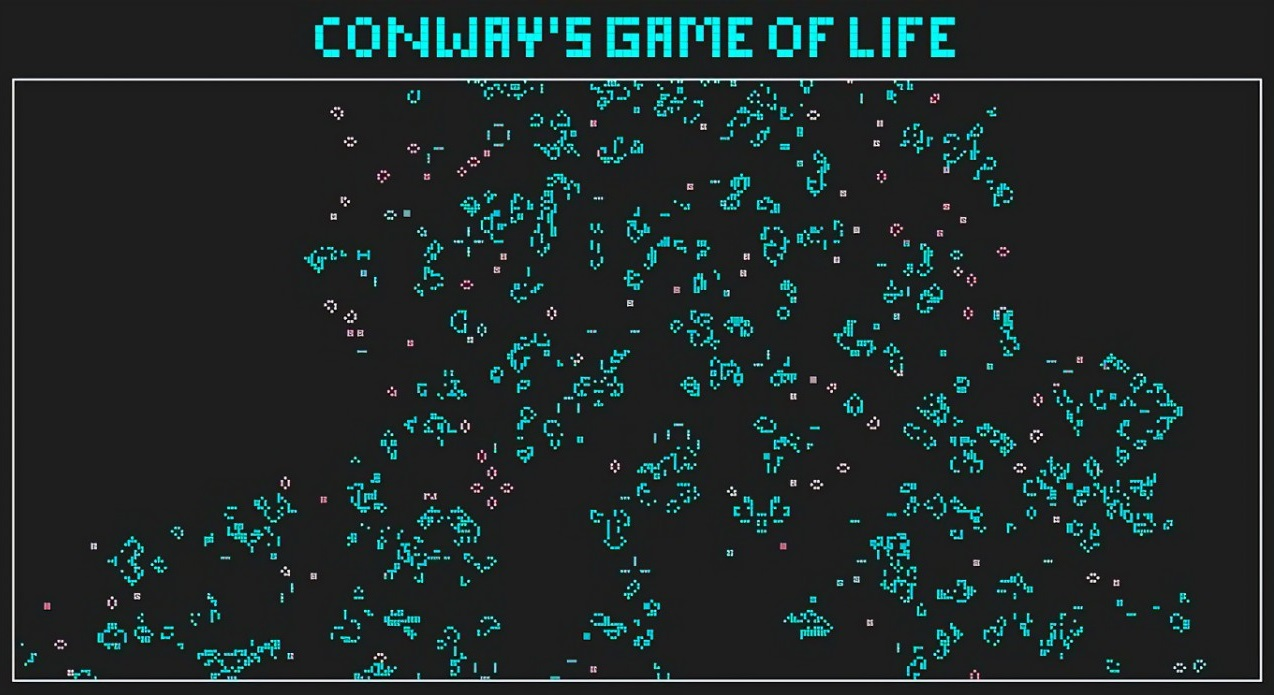
\includegraphics[width=0.75\columnwidth]{figures/gameOfLife.jpg}
		\caption{Conway's Game of Life.}
		\label{fig:figure}
	\end{figure}

    \subsection{Applications}
	
        Cellular automata have been used in various fields, including:
        
        \begin{itemize}
            \item Computer Science: Parallel computation, cryptography, and image processing.
            \item Physics: Modeling physical systems, such as fluid dynamics and crystal growth.
            \item Biology: Simulating biological processes, such as population dynamics and pattern formation.
        \end{itemize}
		
        Fig. \ref{fig:figure} Application of cellular automata on Computer Science.
	\begin{figure}[H]
		\centering
		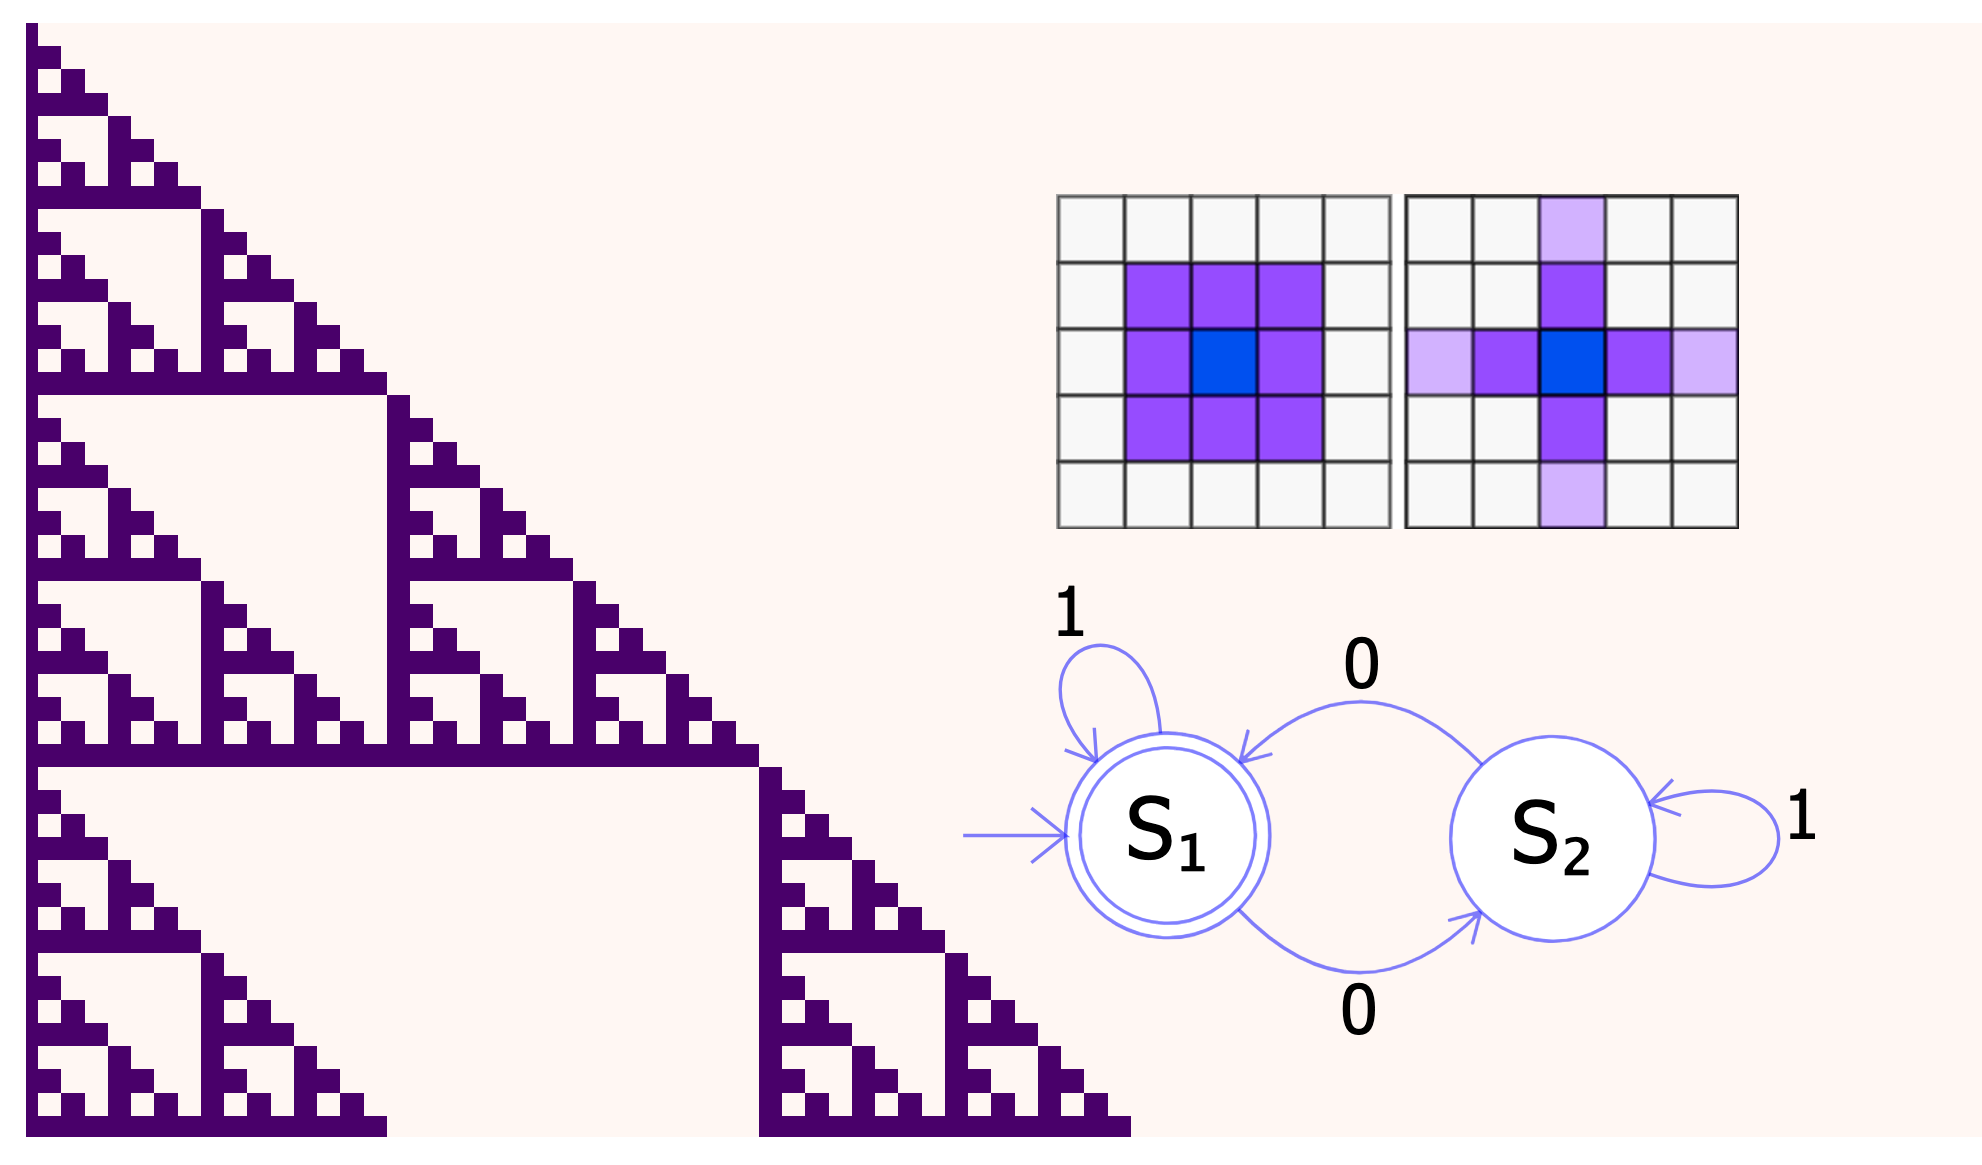
\includegraphics[width=0.75\columnwidth]{figures/theoryOfComputation.png}
		\caption{Example of cellular automata.}
		\label{fig:figure}
	\end{figure}
    \newpage

\section{Cellular Automata Algorithm}

    \begin{algorithm}
        \caption{Basic Cellular Automaton}
        \KwIn{\texttt{gridWidth}: Width of the grid, \texttt{gridHeight}: Height of the grid, \texttt{states}: Set of possibles states for the cells, \texttt{neighborhood}: Set of relative positions defining the neighborhood of each cell, \texttt{rules}: Set of state transition rules, \texttt{maxTimeSteps}: Maximum number of time steps}
        \KwOut{The final state of the grid}
        
        Initialize \texttt{gridHeight} $\times$ \texttt{gridWidth}, set the initial states on the grid and create \texttt{newGrid} as a copy of the grid.\;
        
        \While{$i$ < \texttt{maxTimeSteps}}{
            \For{$x$ in \texttt{gridWidth}}{
                \For{$y$ in \texttt{gridHeight}}{
                    \texttt{neighbors} = getNeighbors(\texttt{grid}, \texttt{neighborhood}, $x$, $y$)\;
                    \texttt{newGrid}[$x$][$y$] = applyRules(\texttt{grid}[$x$][$y$], \texttt{neighbors}, \texttt{rules})\;
                }
            }
            Display the state of \texttt{newGrid}
            \texttt{grid} = \texttt{newGrid}\;
            $i$++\;
        }
        \end{algorithm}

\section{Parameters Required on a Cellular Automata}

\section{Versions of Cellular Automata}

\section{Analogy with the Nature}
    
\section{Implementation Repositories}

\section{Usage Examples}


\end{document}